\subsubsubsubsection{Crossroads}
\begin{figure}[h]
\centering
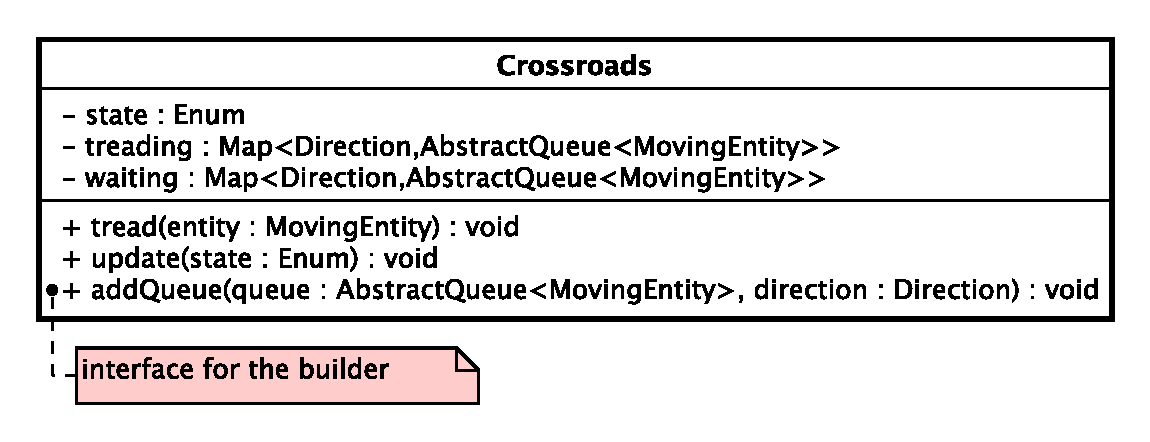
\includegraphics[scale=0.6,keepaspectratio]{images/solution/crossroads.eps}
\caption{App::Reactive::Crossroads}
\label{fig:sd-app-crossroads}
\end{figure}
\FloatBarrier
\begin{itemize}
  \item \textbf{Description} \\
    It represents a concrete crossroads entity. It is a protected object.
  \item \textbf{Attribute}
  \begin{itemize}
    \item \texttt{- state: Enum} \\
The traffic light state indicates which directions to free.
    \item \texttt{- treading: Map<Direction, AbstractQueue<MovingEntity>>} \\
The queue of moving entities which are treading the crossroads.
    \item \texttt{- waiting: Map<Direction, AbstratQueue<MovingEntity>>} \\
The queue of moving entities which are waiting to tread the crossroads. 
  \item \textbf{Operation}
  \begin{itemize} 
    \item \texttt{+ tread(entity: MovingEntity)} \\
Implements the treading of the crossroads.
    \item \texttt{+ update(state: Enum)} \\
Updates the state value of the crossroads.
    \item \texttt{+ addQueue(queue: AbstratQueue<MovingEntity>, direction: Direction)} \\
Add a new queue to waiting and treading maps with the specified direction.
  \end{itemize}
\end{itemize}
